\documentclass[12pt, final]{article}
\usepackage[margin= 0.75in]{geometry}
\usepackage{amsfonts}
\usepackage{amsthm}
\usepackage{amsmath}
\usepackage{mathabx}
\usepackage{ulem}
\usepackage{enumerate}
\usepackage{float}
\usepackage{graphicx}
\graphicspath{{../Code/PLOTS/}}
\usepackage{color}
\usepackage{subcaption}
\usepackage{commath}
\usepackage{caption}

\begin{document}

\captionsetup[figure]{font = footnotesize}
\captionsetup[subfigure]{font = scriptsize}

\newcommand{\Pois}{\text{Pois}}

\newtheorem{prop}{Proposition}


\title{Necessity of STDP and Heterosynaptic Competition in Sequential Firings}
\author{Ansel Blumers and Ankan Ganguly}
\maketitle

\begin{abstract}
Sequential cognitive processing are driven by sequences of neural activity in various parts of the brain. 
Hahnloser \textit{et al.} claim that the combination of heterosynaptic competition within single neurons and spike-time-dependent plasticity (STDP) lead the network to sequential activity. In this paper, we will re-examine their claim by investigating the effect of heterosynaptic competition and the necessity of STDP. We build a model which partially replicates the results of \cite{Fiete}, and demonstrate that these partial properties remain when we replace STDP by Hebbian learning.

\end{abstract}

\newpage

\tableofcontents

\newpage

\section{Introduction}

Vertebrates often need process sequential events. Sequential cognitive processing are driven by sequences of neural activity in various parts of the brain. The ubiquity of repeating sequential neural patterns prompts the speculation that the mechanisms of creation may be general across species. One test subject under frequent investigations is Zebra finch. Zebra finches are songbirds that produce sounds in a recurring fashion.  They can produce motifs that last up to 1 second, while single neuron bursts only sustain about 6 ms. (Hahnoloser \textit{et al.}, 2002)  This leads the conclusion that the coding of sequential activity is sparse. 

The first model seeking to represent neural sequence generation is categorically referred as “synaptic chain” networks (Kleinfeld and Sompolinsky, 1988). The connectivity matrix in such networks is directional – neuronal groups are connected in a single file fashion. However, the network connectivity must be per-defined by hand, severely slashing its usability. 

One attempt to circumvent the drawback was made by Fiete and Hahnloser as described in the article \textit{Spike-Time-Dependent Plasticity and Heterosynaptic Competition Organize Networks to Produce Long Scale-Free Sequences of Neural Activity}. The authors claim that the combination of heterosynpatic competition within single neurons and spike-time-dependent plasticity (STDP) lead the network to sequential activity. 

STDP rules modify the synaptic connection so that the repeated timely causal activation of pair of neurons strengthens the connection, while the reverse is weakened (Bi and Poo, 1998). Synchrony among firings arises naturally as a result. Because of this, a neuron that fires frequently will become a hub that modulates the firings in a network level. To form a long sequence, STDP alone is insufficient as suggested by the authors. Heterosynpatic competition was then introduced to supplement STDP. The underlying idea is  based on cellular biology and well documented - postsynaptic neurons conserve the total synaptic weight by depressing some input synapses when others undergo potentiation (Royer and Pare, 2003). The authors imposed a slightly different implementation onto their model – heterosynaptic long-term depression (hLTD) .


In this paper, we will re-examine Hahnloser et al's claim that the combination of STDP and hLTD give rise to the generation of neural sequential firings. We will first investigate how strong of an effect hLTD imposes on the model by tuning relevant parameter. Then will we inspect the necessity of  STDP. 


\section{Methods}

In this paper, we used the simulated Integrate and Burst (IB) model introduced in \cite{Fiete}. We then implemented STDP learning and Hebbian learning.

\subsection{Integrate and Burst Model}

Our IB model is an implementation of equations described in \cite{Fiete}. We provide a detailed description of those equations here, with more attention paid to the intuition behind these equations. There are \(N\) neurons connected in an all-to-all environment. Each neuron \(i\) bursts when its membrane potential, \(V_i\), hits the threshold \(V_\theta\). We assume that every neuron bursts for \(T_{burst}\) time. While bursting, each neuron fires four times uniformly over the burst interval before resetting to \(V_{reset}\).

When a neuron is not bursting, its potential is governed by a typical conductance based leaky integrate and fire model with built-in inhibition:

\begin{equation}
\tau_V \od{V_i}{t} = -g^L(V - V^L) - g^E_i(V - V^E) - g^I_i(V - V^I)
\label{Potential}
\end{equation}

The leak conductance, \(g^L\), is assumed to be a homogeneous constant input, as is the leak potential \(V^L\). Notice that in the absence of excitatory or inhibitory conductance, neuron \(i\) will tend to \(V^L\). Therefore we can say that the leak potential is also equal to the rest potential.

The excitation potential, \(V^E\), and the inhibition potential, \(V^I\), act as upper and lower bounds on untethered \textcolor{red}{(What was the word for IF potential plots without a firing threshold?)} potential respectively. 

The excitation conductance, \(g^L\), is defined by the activity in neighboring neurons as well by external random stimulation:

\[g^L = Ws + W_0b\]

Where \(W_{ij}\) is the strength of the synapse from neuron \(j\) to neuron \(i\), \(W_0\) is the conductance strength of external synapses and \(b\) is a Poisson random variable with frequency \(r_{in}\). \(r_{in}\) was an input parameter. In \cite{Fiete} \(r_{in}\) was constant, but we chose to assign \(r_{in}\) a high value and anneal it to jump-start neural activity. \(s_i\) is the activation of neuron \(i\). It is incremented each time neuron \(i\) fires, and it decays by

\[\od{s}{t} = -\tau s\]

The inhibitory conductance, \(g^I\), is defined as the sum of the adaptation inhibition, \(g^I_{ada}\), and the global inhibition, \(g^I_{glob}\). The adaptation inhibition is the internal inhibition generated by activation of a neuron. It is defined by the same equations as \(s_i\), but with a constant multiplier \(A_a\) and a slower time-constant \(\tau_{ada}\).

\subsection{Learning}

The purpose of this paper is to replicate and test some of the claims made in \cite{Fiete}. One of the claims made is that the model used by \cite{Fiete} demonstrates how STDP can contribute to the synchronous regular synfiring chains exhibited in Zebra Finch \textcolor{red}{(Where? Maybe cite second paper here?)}. We implemented STDP, but we also implemented a pure Hebbian learning rule to demonstrate that STDP learning is not necessary for the model to exhibit synchronous regular firing chains.

\subsubsection{STDP Learning}

We followed \cite{Fiete} precisely in our implementation of STDP learning. Define

\[K(t) = 
\begin{cases}
e^{-t/\tau_{STDP}} &\text{ if } t > 0\\
-e^{-t/\tau{STDP}} &\text{ if } t < 0\\
0 &\text{ otherwise}
\end{cases}
\]

as the STDP kernel. For every pair of neurons \(i,j\), let \(t_i < t_j\) be two times when \(i\) and \(j\) fired respectively. Then According to STDP, the weight matrix element \(W_{ij}\) should increase proportional to \(K(t_j - t_i)\). Notice that the change in \(W\) according to STDP is approximately anti-symmetric. \cite{Fiete} strengthened the nonlinearity of STDP by making STDP growth of a synapse proportional to the strength of that synapse (with an added factor so 0 weight synapses could grow). In particular, the paper defined:

\begin{equation}
\Delta^{STDP}_{ij}(t) = \left(\frac{W_{ij}(t-1)}{w_{max}} + 0.001\right)*\left(x_i(t)K(0)x_j(t) + \sum_{\tau = 0}^t  [x_i(t)K(\tau)x_j(t -\tau) - x_i(t - \tau)K(\tau)x_j(t)]\right)
\label{STDP}
\end{equation}

Where \(x_i(t)\) is a binary variable taking the value 1 if neuron \(i\) fired at time \(t\). So, at each time \(t\), \(\Delta^{STDP}(t)\) is proportional to the change in \(W\) with respect to STDP. Our implementation assumed \(K(t) \approx 0\) for \(t > 4\)ms.

However, the key innovation of this paper was to introduce a secondary source of competition. If the total strength of all synapses into or out of a given neuron exceed a soft limit \(W_{max}\) after STDP learning, then all such synapses experience long-term depression (LTD) proportional to the amount by which the soft limit is exceeded:

\begin{equation}
\theta^{col}_i =  \left[\sum_{j=1}^N (W_{ij} + \eta\Delta^{STDP}_{ij}) - W_{max}\right]^+
\label{hLTP}
\end{equation}

\(\theta^{col}\) denotes the amount by which the soft limit has been exceeded. Define \(\theta^{row}\) similarly. Then,

\begin{equation}
\od{W_{ij}}{t} = \eta\Delta^{STDP}_{ij} - \epsilon(\theta^{col}_i + \theta^{row}_j)
\label{Learning}
\end{equation}

This updates weights according to STDP along with a penalty if the soft limit is exceeded. Finally, to ensure that STDP never diverges, we implement a hard limit. If any element \(W_{ij}(t) > w_{max}\), where \(w_{max}\) is a constant parameter, we manually set \(W_{ij}(t)\) to \(w_{max}\). 

We actually implemented the results incorrectly based on a typo in \cite{Fiete}. Our implementation used the following equations:

\begin{equation}
\theta^{col}_i =  \left[\sum_{j=1}^N (W_{ij} + \Delta^{STDP}_{ij}) - W_{max}\right]^+
\label{hLTP-wrong}
\end{equation}

\begin{equation}
\od{W_{ij}}{t} = \eta\Delta^{STDP}_{ij} - \eta\epsilon(\theta^{col}_i + \theta^{row}_j)
\label{Learning-wrong}
\end{equation}

As demonstrated in sections 3 and 4, this causes some significant issues with convergence. Unfortunately, we noticed the problem too late into the project to redo the simulations.

\subsubsection{Hebbian Learning}

Hebbian plasticity is a general family of learning rules which strengthen synapses between neurons which fire with high correlation. Hebbian learning rules are generally considered incomplete because while they explain how synapses are strengthened, they do not explain how synapses might be weakened. 

One way to complete the Hebbian learning rule is with STDP. In STDP learning, highly correlated neurons experience a large change in synaptic strength, but the direction of the change (increase or decrease) depends on the relative timing of firing between the synapses.

However, the soft and hard limits imposed by the model also provide a way for synapse strength to decrease, so it should be possible to implement this model using Hebbian plasticity. To do this, we ran the exact same learning algorithm as implemented for STDP, but we modified the kernel to be

\[K(t) = 
\begin{cases}
e^{-t/\tau_{Heb}} &\text{ if } t > 0\\
0 &\text{ otherwise}
\end{cases}
\]

With this new kernel, 

\begin{equation}
\Delta^{Heb}_{ij}(t) = \left(\frac{W_{ij}(t-1)}{w_{max}} + 0.001\right)*\left(x_i(t)K(0)x_j(t) + \sum_{\tau = 0}^t  x_i(t)K(\tau)x_j(t -\tau)\right)
\label{Heb}
\end{equation}

gives us a Hebbian learning rule. We implemented the soft and hard synaptic weight limits as in STDP learning.

\subsection{Parameter Choices}

Our implementation of the IB neuron network with STDP learning matched that used in \cite{Fiete} in many cases. However a few parameters were chosen differently. The table below provides a list of parameters we used:

\begin{center}
\begin{tabular}{|c|c|p{0.5cm}|c|c|p{0.5 cm}|c|c|}
\cline{1-2}\cline{4-5}\cline{7-8}
Parameters & Values & & Parameters & Values& & Parameters& Values\\

\cline{1-2}\cline{4-5}\cline{7-8}
\(dt\) & \(2 \times 10^{-5}\)s& & \(\tau_V\) & 0.01 F/m\(^2\)& &\(V^L\) & -0.06V\\

\cline{1-2}\cline{4-5}\cline{7-8}
\(V^E\) & 0V& & \(V^I\) & -0.07V& & \(W_0\) & 5S/m\(^2\)\\

\cline{1-2}\cline{4-5}\cline{7-8}
\(V_{\theta}\) & -0.05V & & \(V_{reset}\) & -0.055V & & \(T_{burst}\) & 0.006s\\

\cline{1-2}\cline{4-5}\cline{7-8}
\(\tau\) & 0.004s & & \(r_{in}^{start}\) & 10000Hz & & \(r_{in}^{min}\) & 4000Hz, 6000Hz\\

\cline{1-2}\cline{4-5}\cline{7-8}
\(N\) & 50 & & \(w_{max}\) & 0.14 & & \(W_{max}\) & 0.14\\

\cline{1-2}\cline{4-5}\cline{7-8}
\(\eta\) & varies & & \(\epsilon\) & varies & & \(A_g\) & 4\\

\cline{1-2}\cline{4-5}\cline{7-8}
\(A_a\) & 9 & & \(\tau_{STDP}= \tau_{Heb}\) & 0.02s & & \(\tau_{ada}\) & 0.015s\\
\cline{1-2}\cline{4-5}\cline{7-8}
\end{tabular}
\end{center}

\section{Results}

We were primarily interested in two major results produced in \cite{Fiete}. First, we were interested the occurrence of long synfire chains with synchronous regular firing. We also investigated the paper's claim that STDP learning with \(w_{max} = W_{max}\) converged to scaled permutation matrices.

Though we tried to replicate the algorithm described in \cite{Fiete}, we were unable to produce a stable system with the provided inputs, so we had to tune the parameters a bit. We eventually found parameters at which burst rates were steady and believable. 

With the parameters we found, we were able to observe weaker versions of most of the observations in the paper. We found that weight matrices converged near permutation matrices and we were able to observe some short sequences of firing chains, but we did not see the synchronous regular behavior exhibited in the paper.

Finally, we replaced STDP learning with Hebbian learning and demonstrated that the weights of a system undergoing Hebbian learning with soft and hard limits converged as closely or better to permutation matrices than they did under STDP learning.

\subsection{Parameter Tuning}

Although our model was constructed to be identical to the model used in \cite{Fiete}, we were unable to use the same parameters as the paper. As an example, the paper claimed to set \(r_{in}\), external input, at 4 Hz. At 4 Hz, we were unable to get our system to fire at all! We assumed it was a typo (the rest of the parameters were given in terms of ms), and attempted running our simulation at 4000Hz. Even 4000Hz was not enough to get the system started, so we tried simulated annealing. The system began with 10000Hz of stimulation, which decreased steadily to 4000Hz. We did this again, but this time stopped at 6000Hz. The difference was striking (see figure \ref{burstSTDP}). 

\begin{figure}[H]
\centering
\begin{subfigure}[b]{0.49\textwidth}
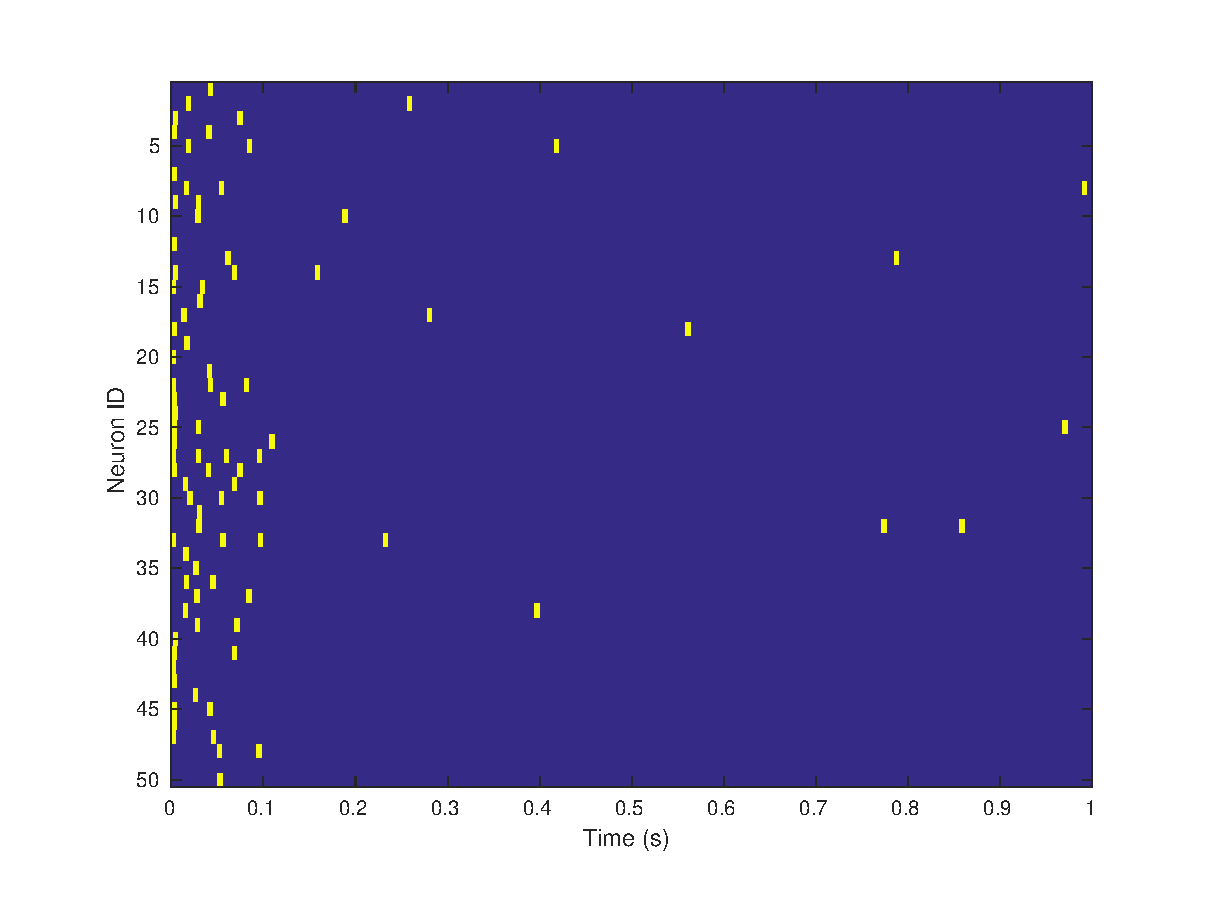
\includegraphics[width=\textwidth]{Burst_plot_4000Hz.eps}
\caption{4000 Hz}
\label{burstSTDP:4000}
\end{subfigure}
\,
\begin{subfigure}[b]{0.49\textwidth}
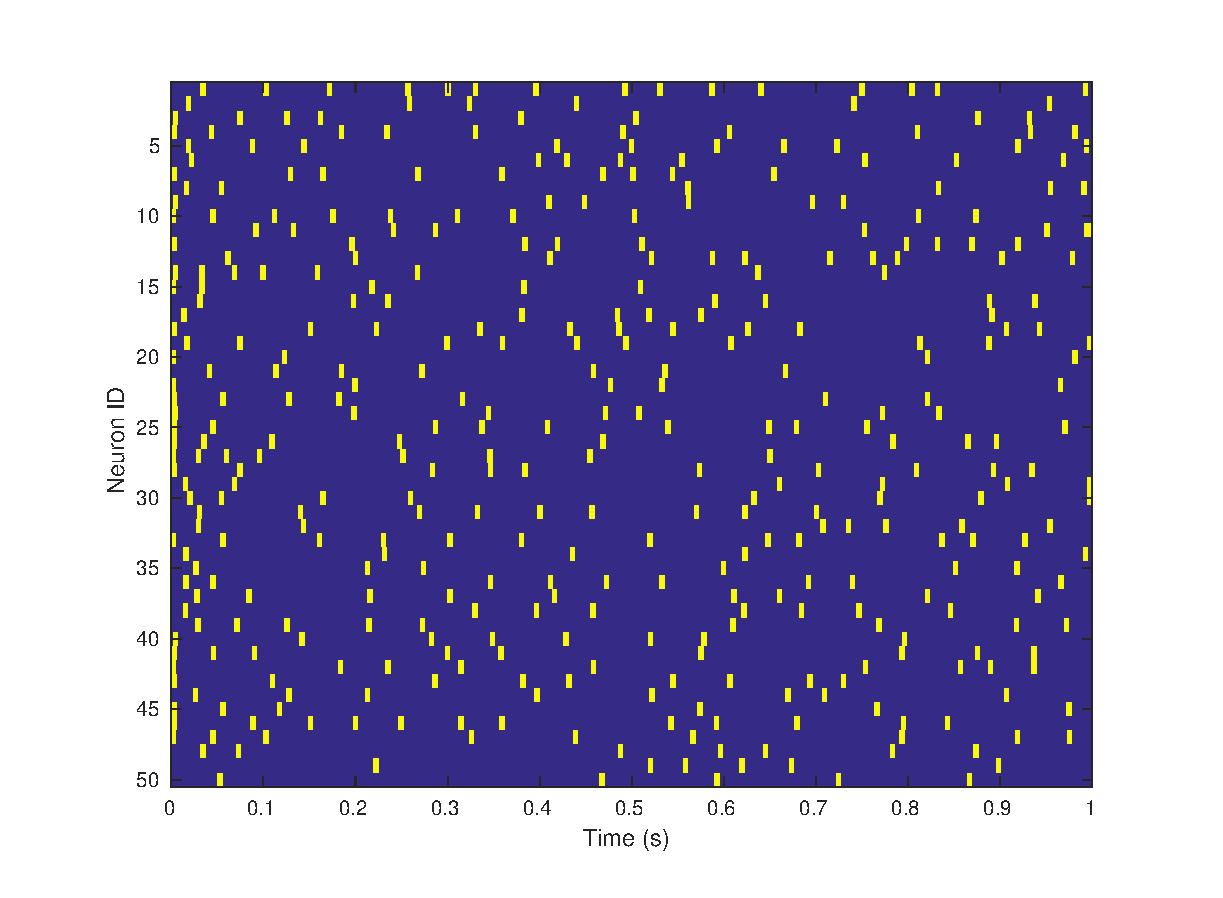
\includegraphics[width=\textwidth]{Burst_plot_6000Hz.eps}
\caption{6000 Hz}
\label{burstSTDP:6000}
\end{subfigure}
\caption{In figure 4 of \cite{Fiete}, the authors displayed a burst plot in which each neuron burst every 75 ms with high synchrony and regularity. We did not observe such synchrony in either plot, but the average frequency of firing in (b) was approximately 75 ms. Notice both systems exhibited exaggerated firing in the beginning. This was a consequence of simulated annealing.}
\label{burstSTDP}
\end{figure}

Beside \(r_{in}\), we spent a lot of time finding appropriate values for \(\eta\) and \(\epsilon\). 

\(\eta\) is the learning step-size. If \(\eta\) is too small, the weight matrix will not converge in a reasonable amount of time. If it is too large, whenever the weight matrix overshoots the soft limit, it will do so by a large margin, which will prompt large corrective measures, so convergence to a permutation matrix (which is barely under the soft limit), will not be plausible.
 
\(\epsilon\) is the strength of the soft limit. If \(\epsilon\) is too small, then when the weight matrix passes the soft limit it will not experience very strong hLTD. This will have the effect of weakening heterosynaptic competition. If \(\epsilon\) is too large, then each time the weight matrix passes the soft limit, it will experience very strong hLTD. Because the permutation matrix is on the border of the soft limit, having a large \(\epsilon\) will make any permutation matrix an unstable critical point in our simulation.

To evaluate these, we ran the simulation on a large combination of parameter values for \(r_{in}, \eta\) and \(\epsilon\). For each of these, we tested convergence using an error function (see section 3.2). The results are shown below:

\begin{figure}[H]
\centering
\begin{subfigure}[b]{0.49\textwidth}
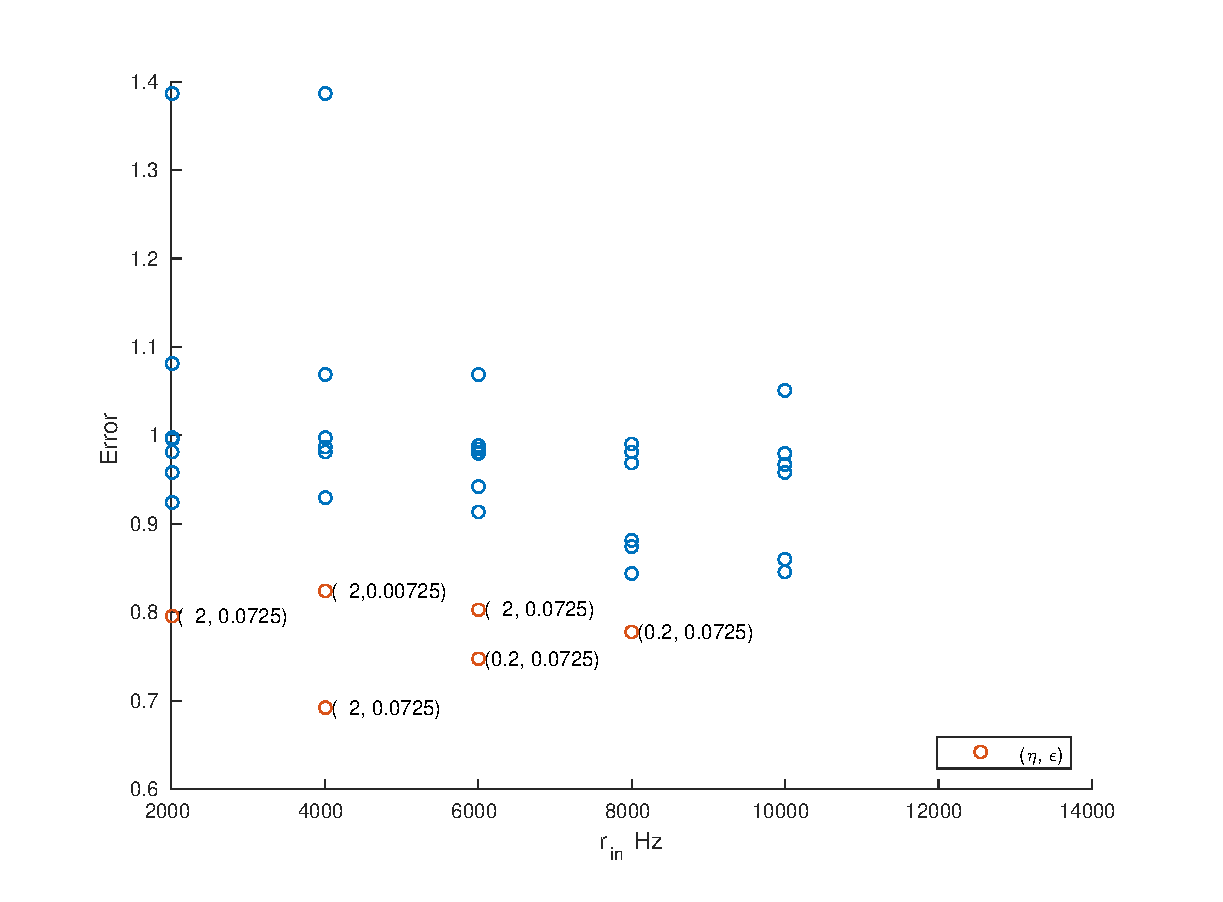
\includegraphics[width = \textwidth]{Error_Scatter_all.eps}
\label{Error_scatter: all}
\caption{Errors of all simulations run}
\end{subfigure}
\,
\begin{subfigure}[b]{0.49\textwidth}
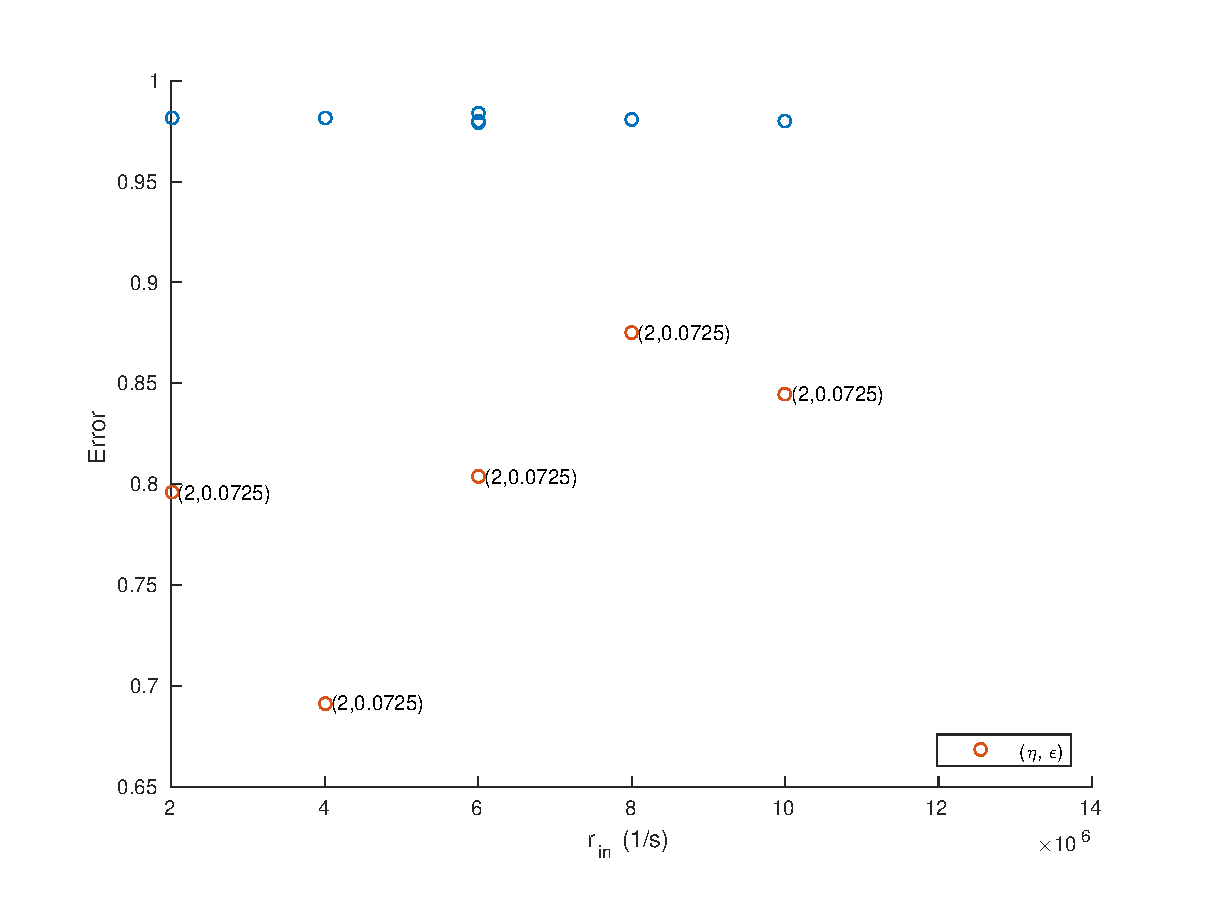
\includegraphics[width = \textwidth]{Error_Scatter_constantproduct.eps}
\label{Error_scatter: constant product}
\caption{Scatterplot of all errors with constant product}
\end{subfigure}
\label{Error_scatter}
\caption{Compare the two}
\end{figure}

Setting \(w_{max}\). (Burst History)

\begin{figure}[H]
\centering
\begin{subfigure}[b]{0.49\textwidth}
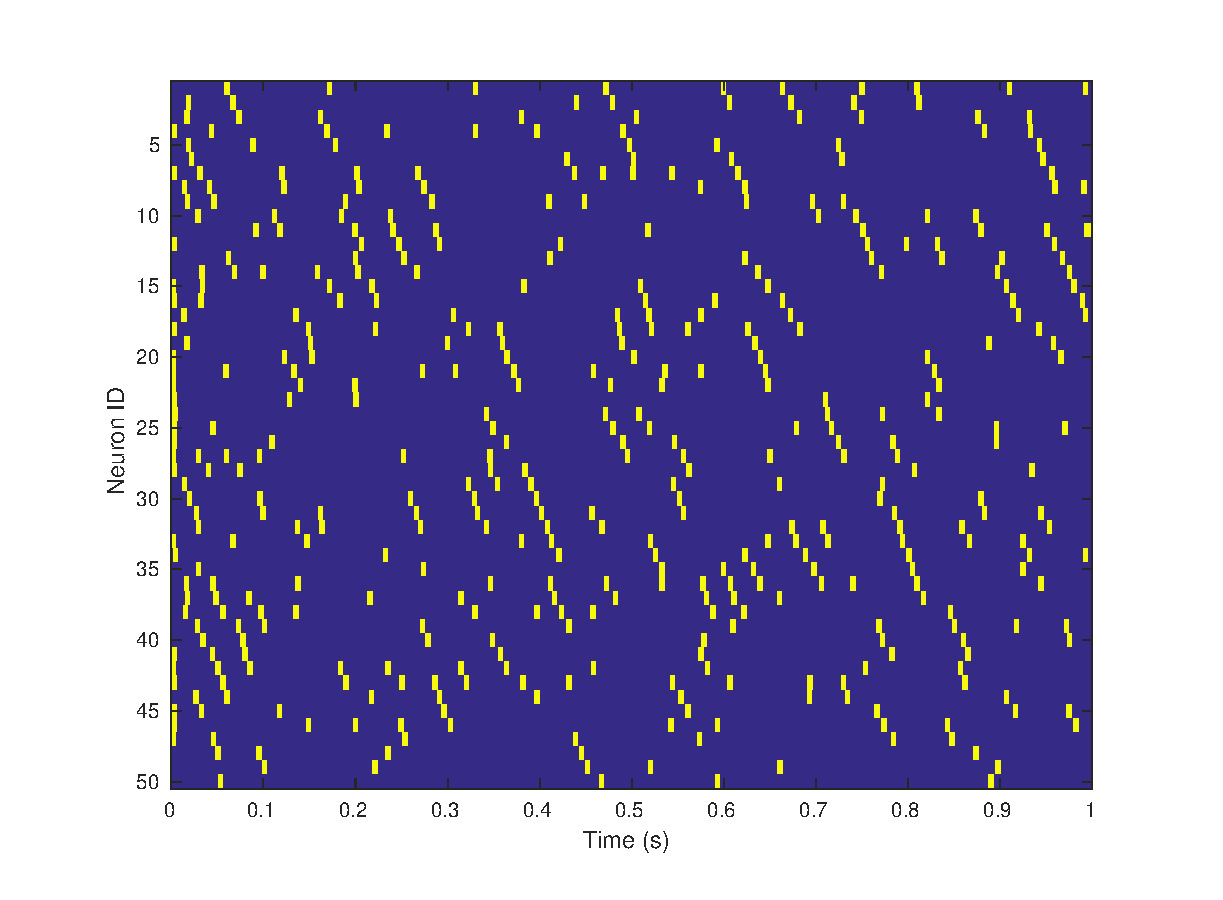
\includegraphics[width = \textwidth]{Burst_nolearning_perm_6000Hz_wmax0.14.eps}
\label{Burst_no_learning: 0.14}
\caption{Bursts without learning, \(w_max = 0.14\).}
\end{subfigure}
\,
\begin{subfigure}[b]{0.49\textwidth}
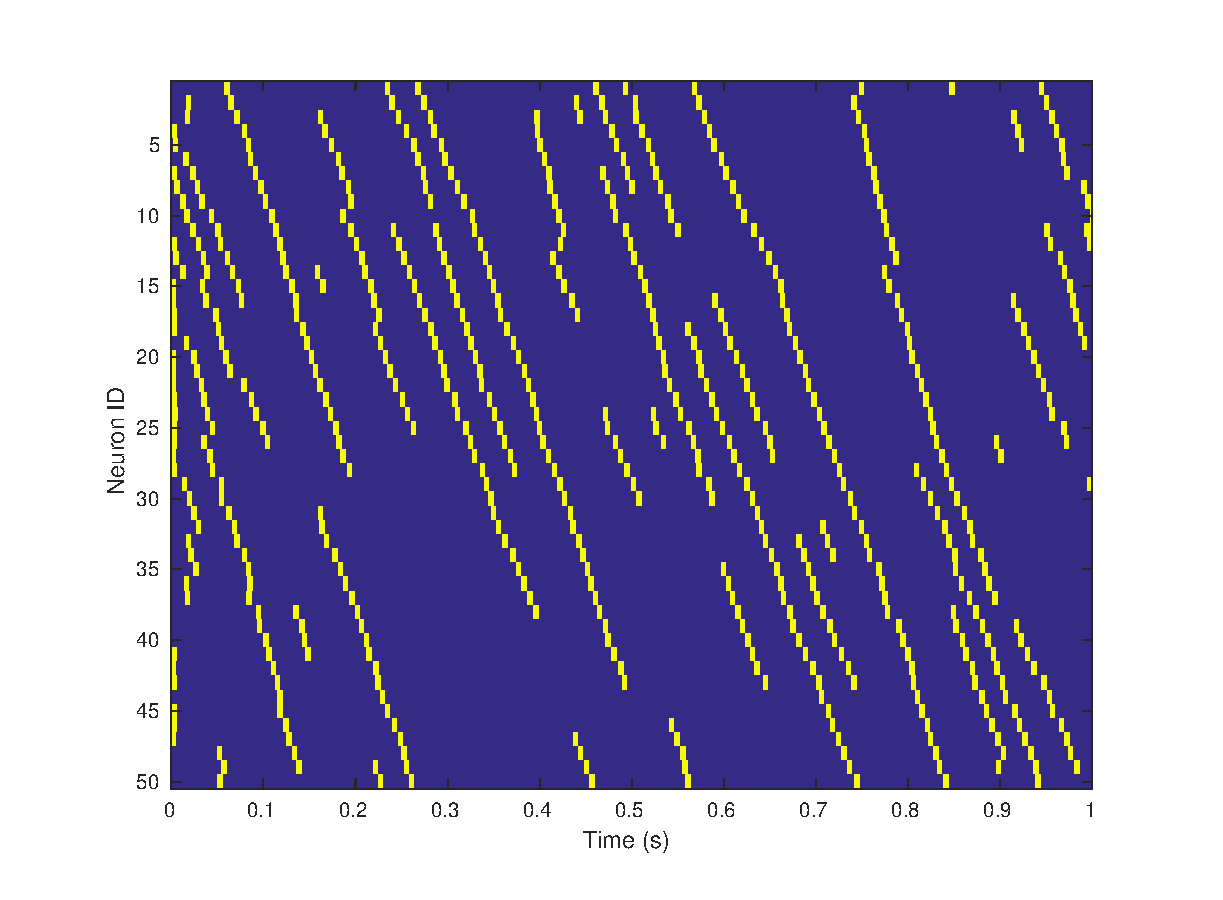
\includegraphics[width = \textwidth]{Burst_nolearning_perm_6000Hz_wmax0.3.eps}
\label{Burst_no_learning: 0.3}
\caption{Bursts without learning, \(w_max = 0.3\).}
\end{subfigure}
\\
\begin{subfigure}[b]{0.49\textwidth}
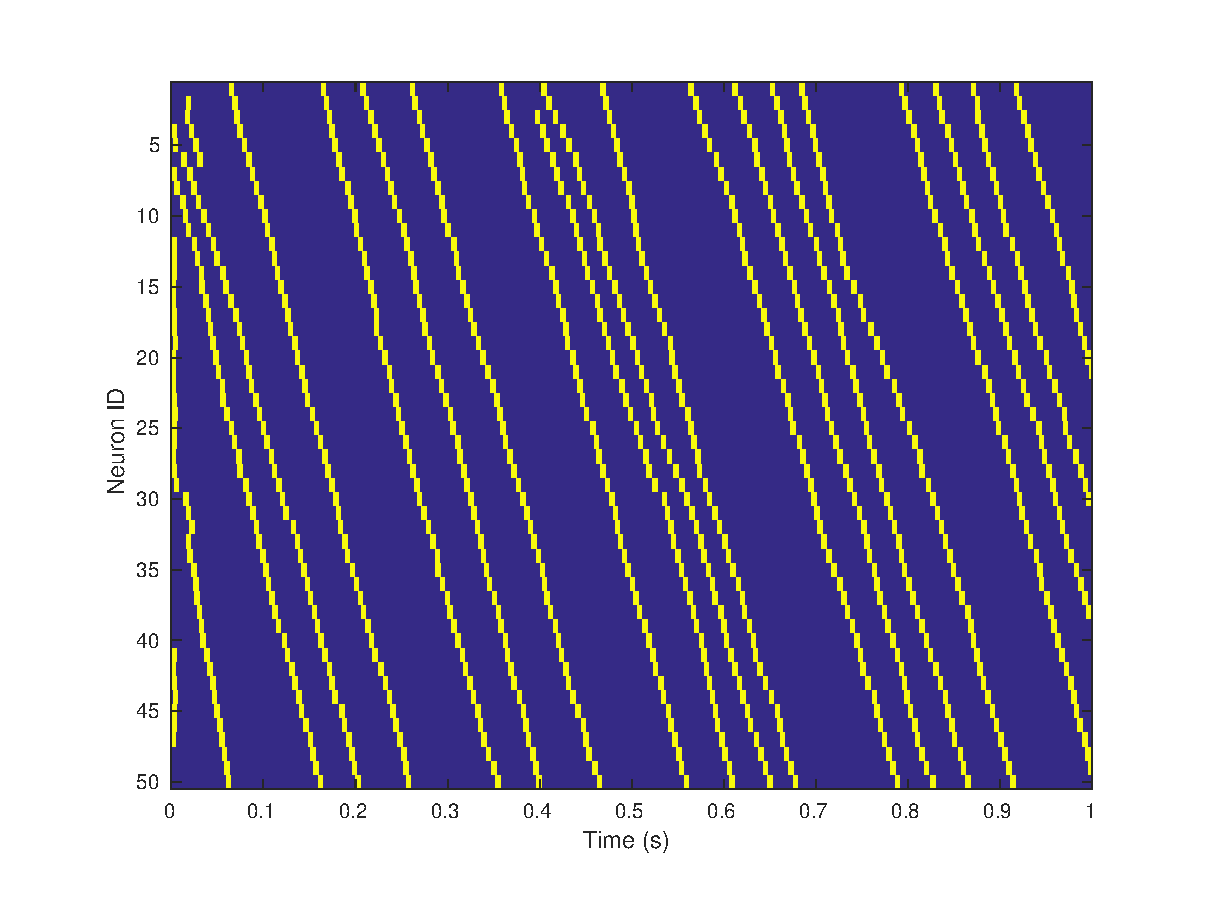
\includegraphics[width = \textwidth]{Burst_nolearning_perm_6000Hz_wmax0.5.eps}
\label{Burst_no_learning: 0.5}
\caption{Bursts without learning, \(w_max = 0.5\).}
\end{subfigure}
\,
\begin{subfigure}[b]{0.49\textwidth}
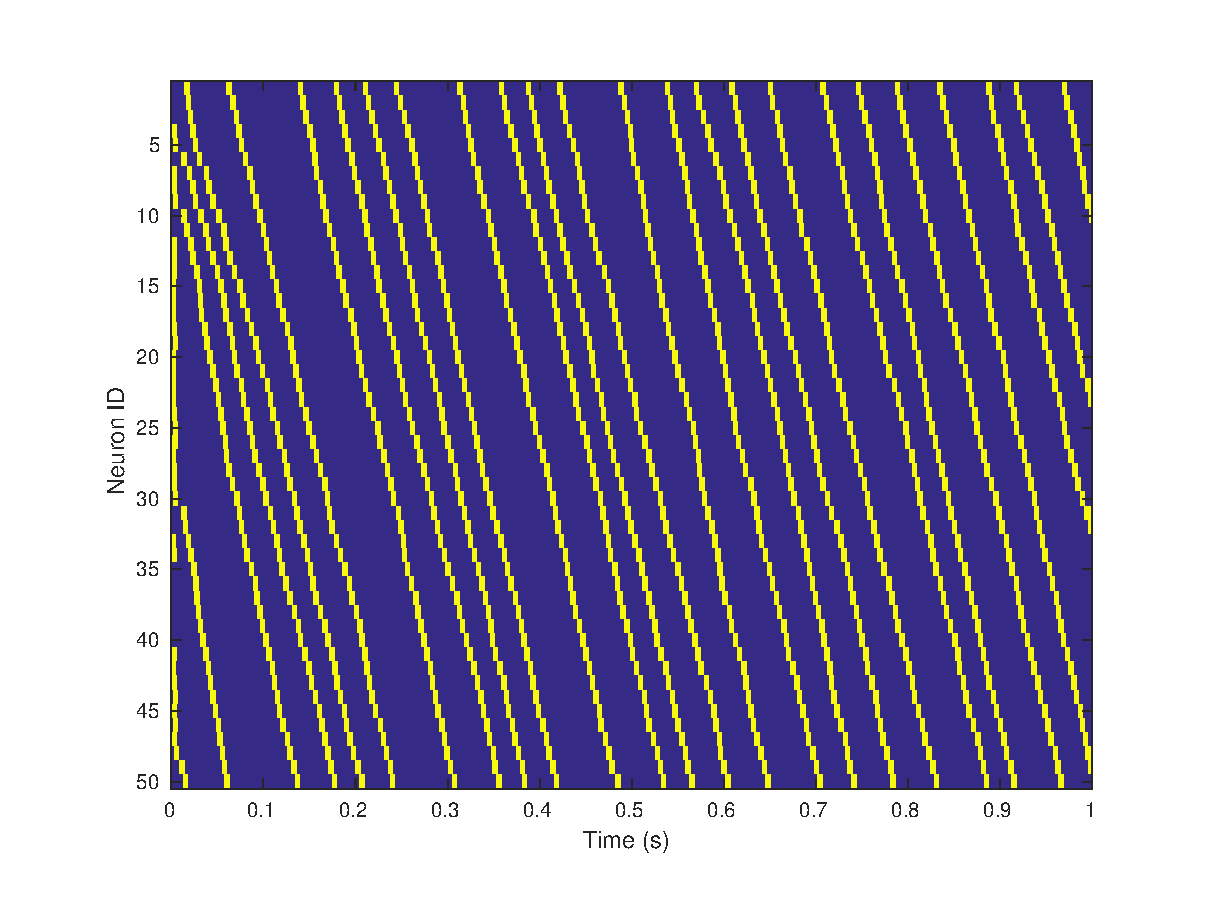
\includegraphics[width = \textwidth]{Burst_nolearning_perm_6000Hz_wmax0.7.eps}
\label{Burst_no_learning: 0.7}
\caption{Bursts without learning, \(w_max = 0.7\).}
\end{subfigure}
\label{Burst_no_learning}
\caption{Compare the four}
\end{figure}


\subsection{Convergence and Stability}

\begin{itemize}
\item Demonstrate the stability of our IB model by showing the firing rate plot and how it splits according to \(r_{in}\).

\begin{figure}[H]
\centering
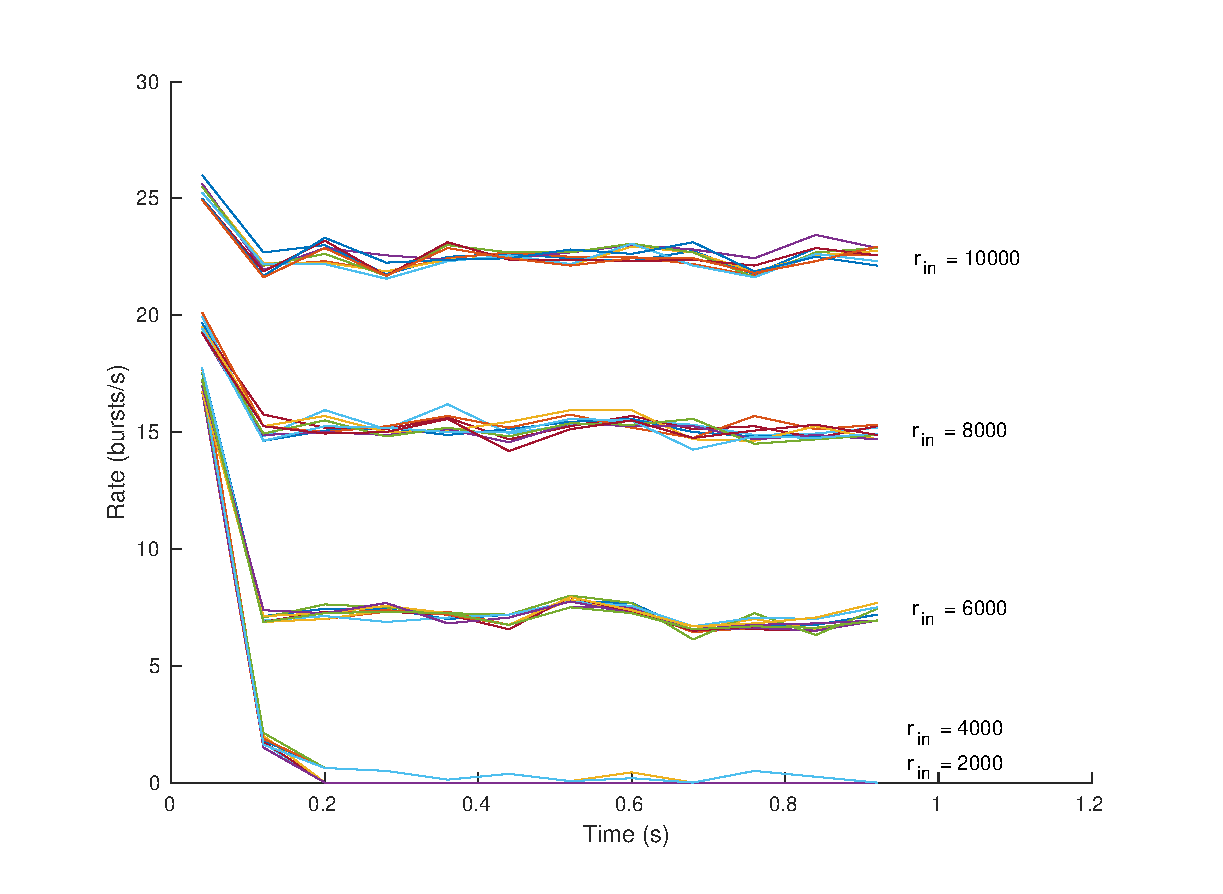
\includegraphics[scale = 0.4]{Firing_Rate_Binsize_80ms.eps}
\label{FR}
\caption{Caption will go here}
\end{figure}

\item Plot Weight and \(WW^T\) for 4000 and 6000 Hz to show some level of convergence.

\begin{figure}[H]
\centering
\begin{subfigure}[b]{0.49\textwidth}
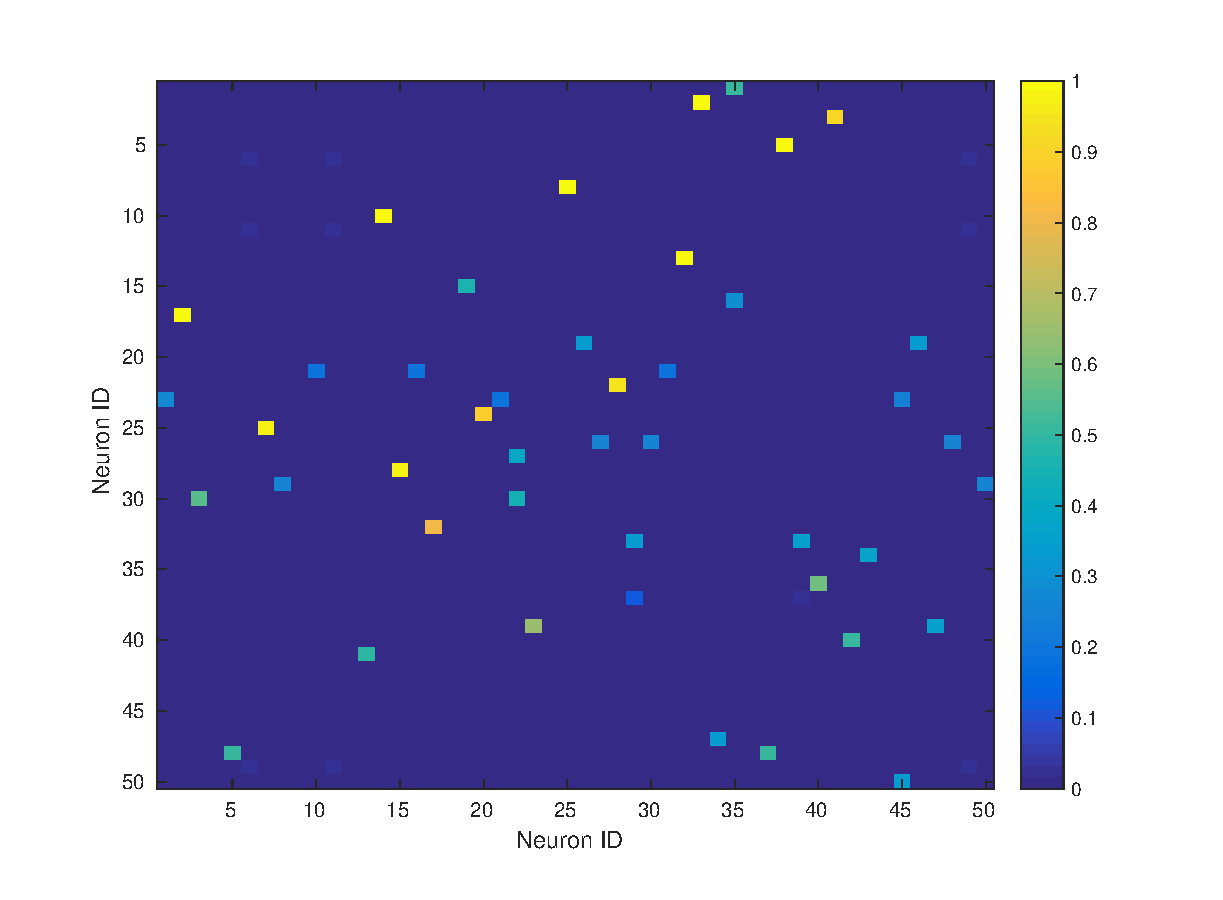
\includegraphics[width = \textwidth]{Weights_4000Hz.eps}
\label{Weights: 4000Hz, basic}
\caption{Weight matrix of 4000Hz annealed}
\end{subfigure}
\,
\begin{subfigure}[b]{0.49\textwidth}
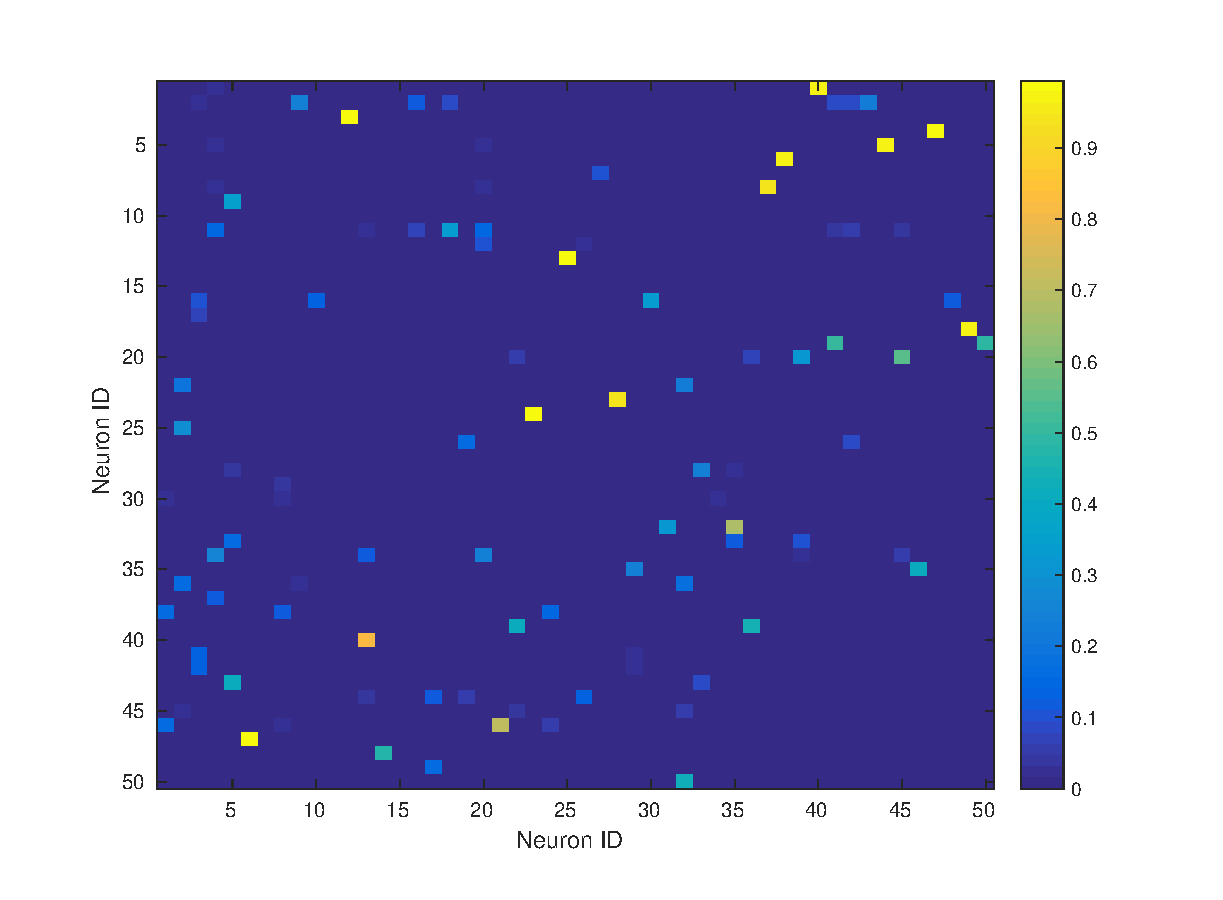
\includegraphics[width = \textwidth]{Weights_6000Hz.eps}
\label{Weights: 6000Hz, basic}
\caption{Weight matrix of 6000Hz annealed}
\end{subfigure}
\\
\begin{subfigure}[b]{0.49\textwidth}
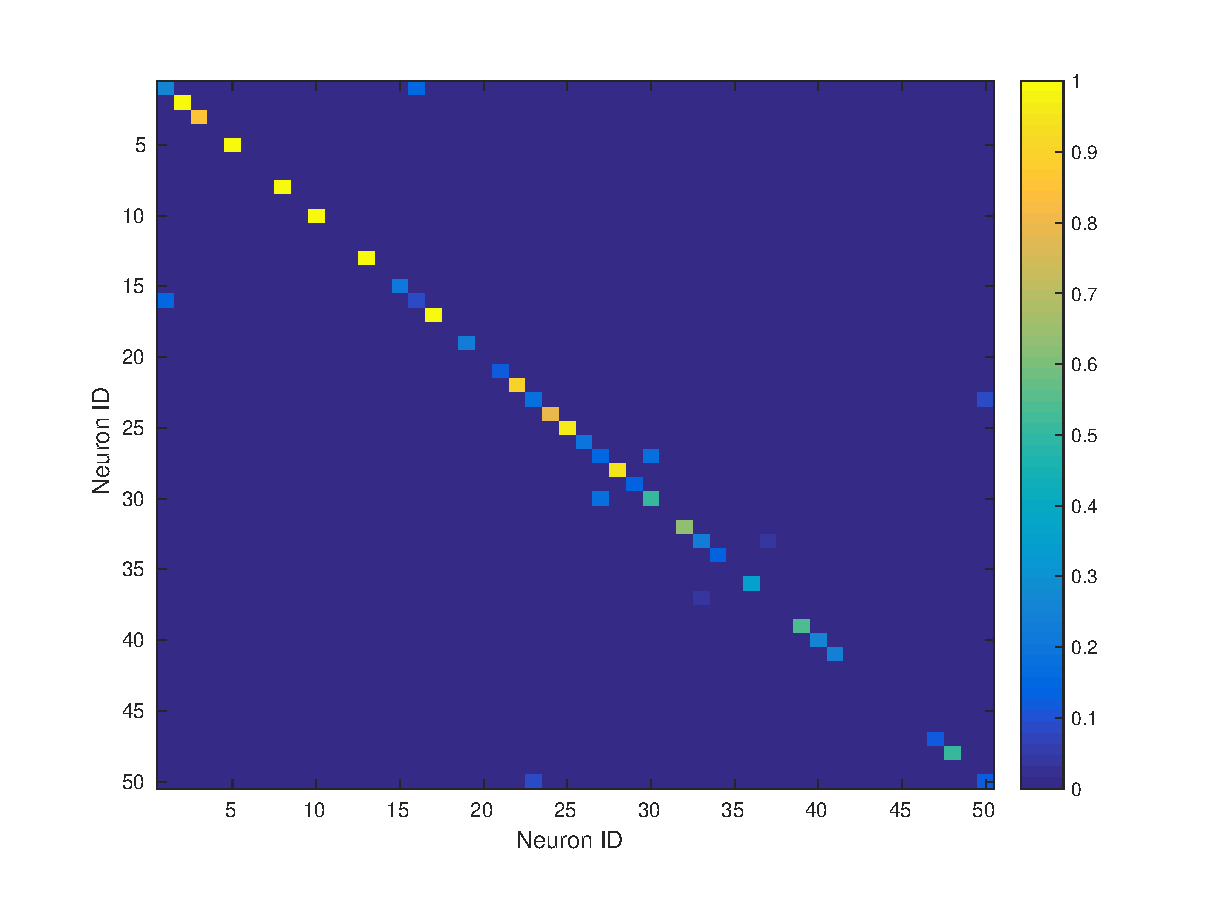
\includegraphics[width = \textwidth]{WW_4000Hz.eps}
\label{Weights: 4000Hz, product}
\caption{\(WW^T\) of 4000Hz annealed}
\end{subfigure}
\,
\begin{subfigure}[b]{0.49\textwidth}
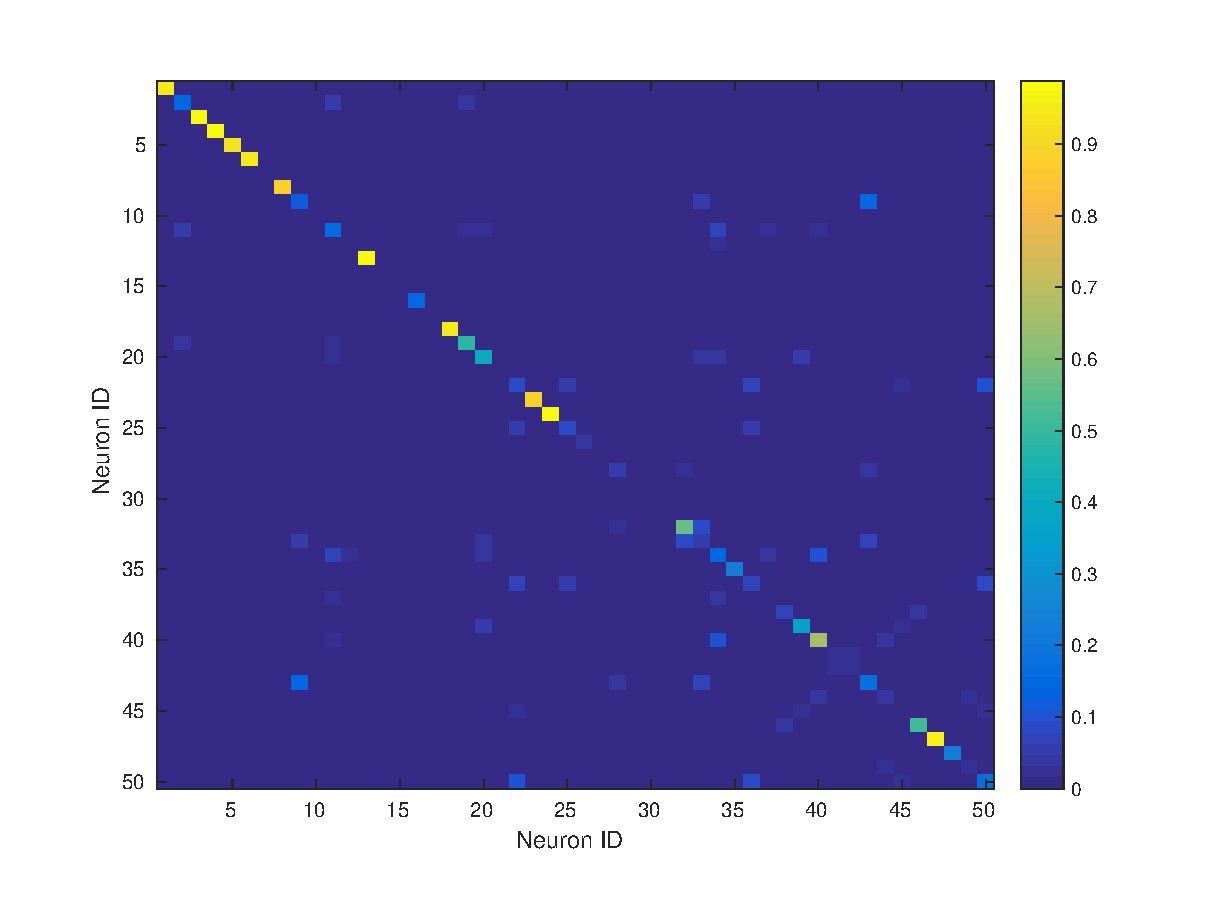
\includegraphics[width = \textwidth]{WW_6000Hz.eps}
\label{Weights: 6000Hz, product}
\caption{\(WW^T\) of 6000Hz annealed}
\end{subfigure}
\label{Weights}
\caption{Compare the four}
\end{figure}

\item Plot error function over time from normal and from permutation matrix

\begin{figure}[H]
\centering
\begin{subfigure}[b]{0.49\textwidth}
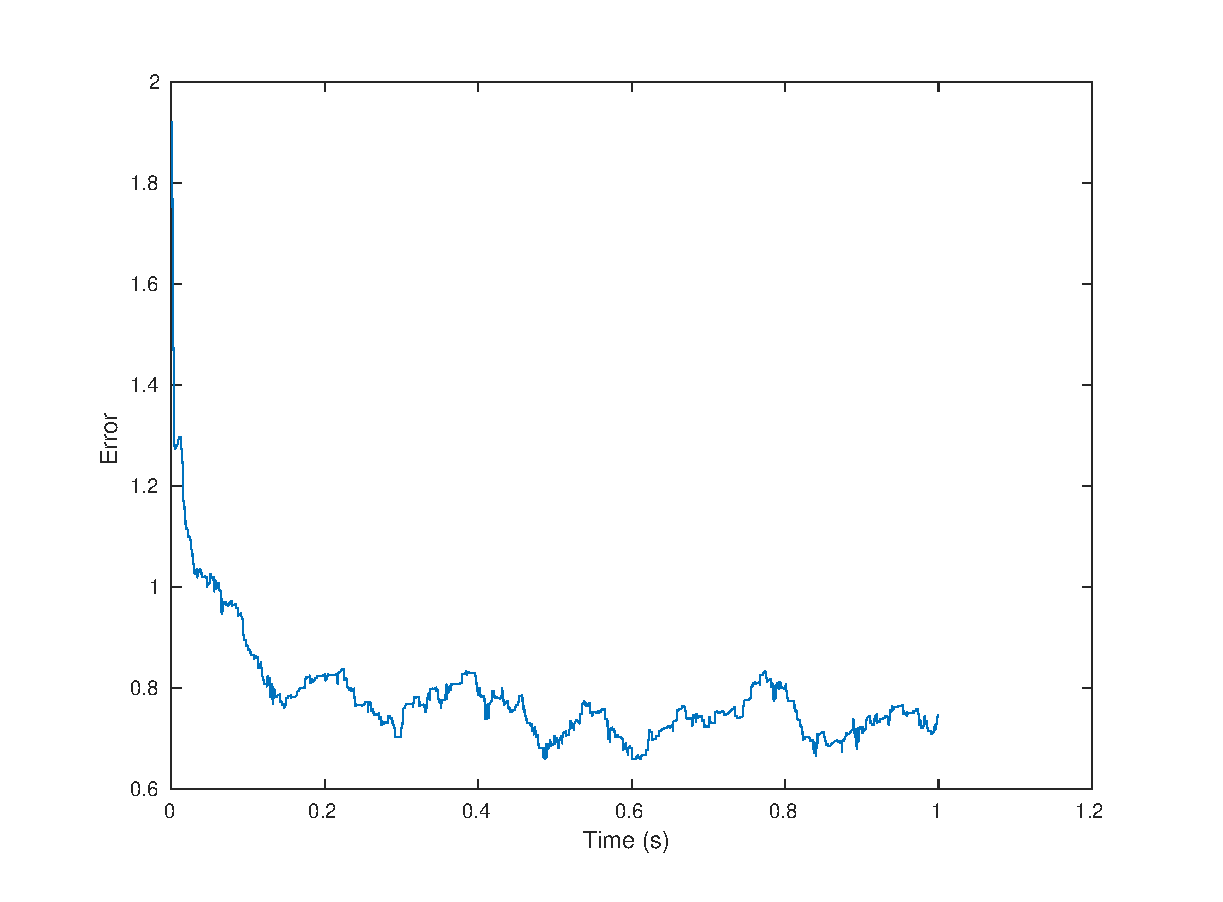
\includegraphics[width = \textwidth]{ErrorOverTime_6000Hz_normal.eps}
\label{Error_over_time: normal}
\caption{Plot of error in weights over time starting from a full connection weight matrix.}
\end{subfigure}
\,
\begin{subfigure}[b]{0.49\textwidth}
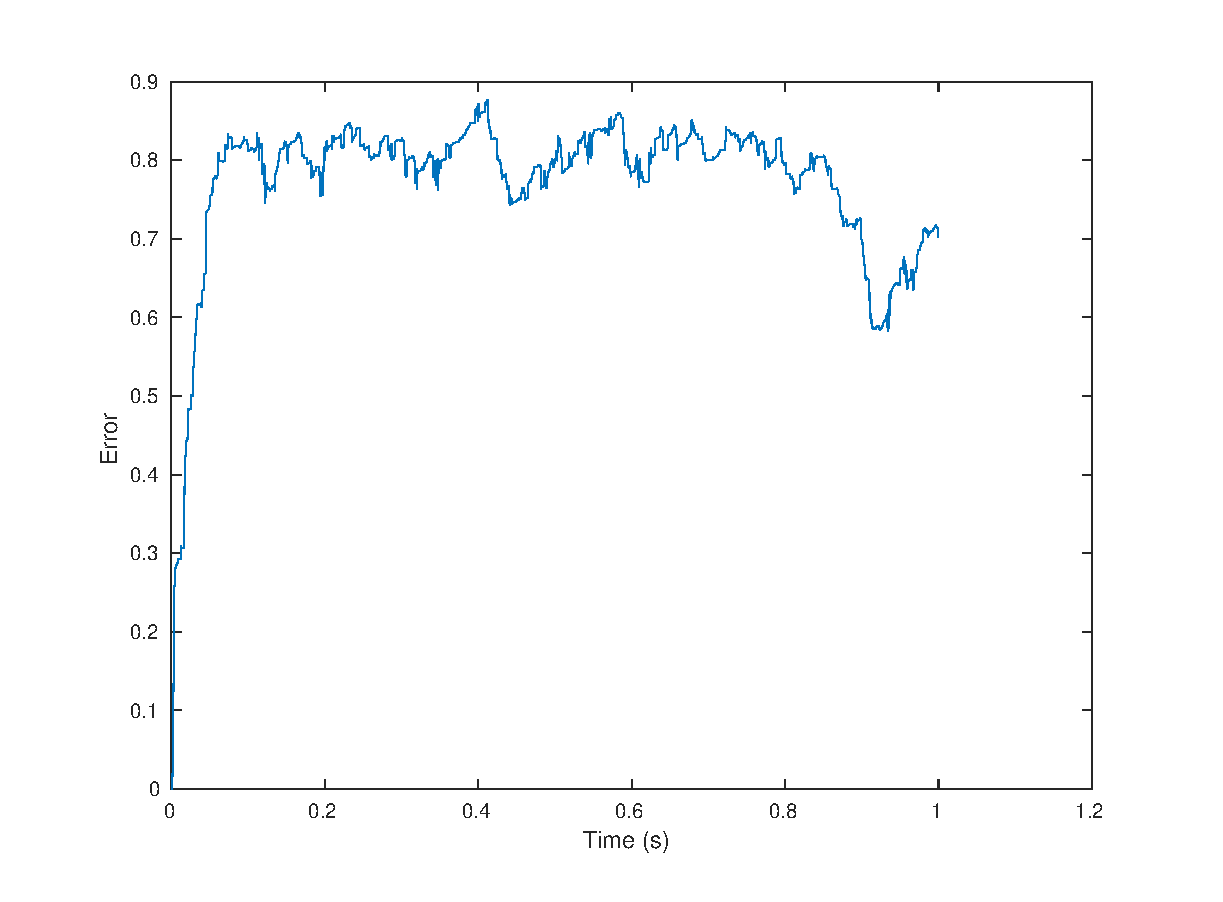
\includegraphics[width = \textwidth]{ErrorOverTime_6000Hz_Perm.eps}
\label{Error_over_time: permutation}
\caption{Plot of error in weights over time starting from a permutation weight matrix.}
\end{subfigure}
\label{Error_over_time}
\caption{Compare the two}
\end{figure}

\item Describe why the error function converges away from (mistake, see discussion).
\end{itemize}

\subsection{Hebbian Learning versus STDP}

\begin{itemize}
\item Introduce the idea of the refutation. 
\item Give a theoretical description why the type of learning should be relatively unimportant.
\item Compare plots (\(WW^T\), Error vs Time, Burst History).

\begin{figure}[H]
\centering
\begin{subfigure}[b]{0.49\textwidth}
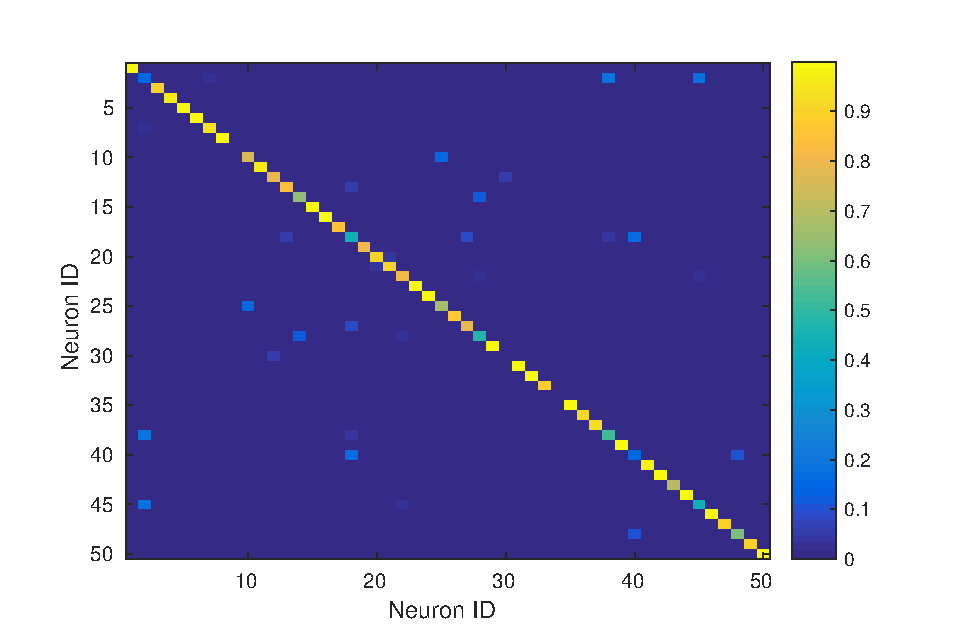
\includegraphics[width = \textwidth]{WW_6000Hz_Hebbian.eps}
\label{Compare: WW_Hebbian}
\caption{Multiplied weight matrix with Hebbian learning}
\end{subfigure}
\,
\begin{subfigure}[b]{0.49\textwidth}
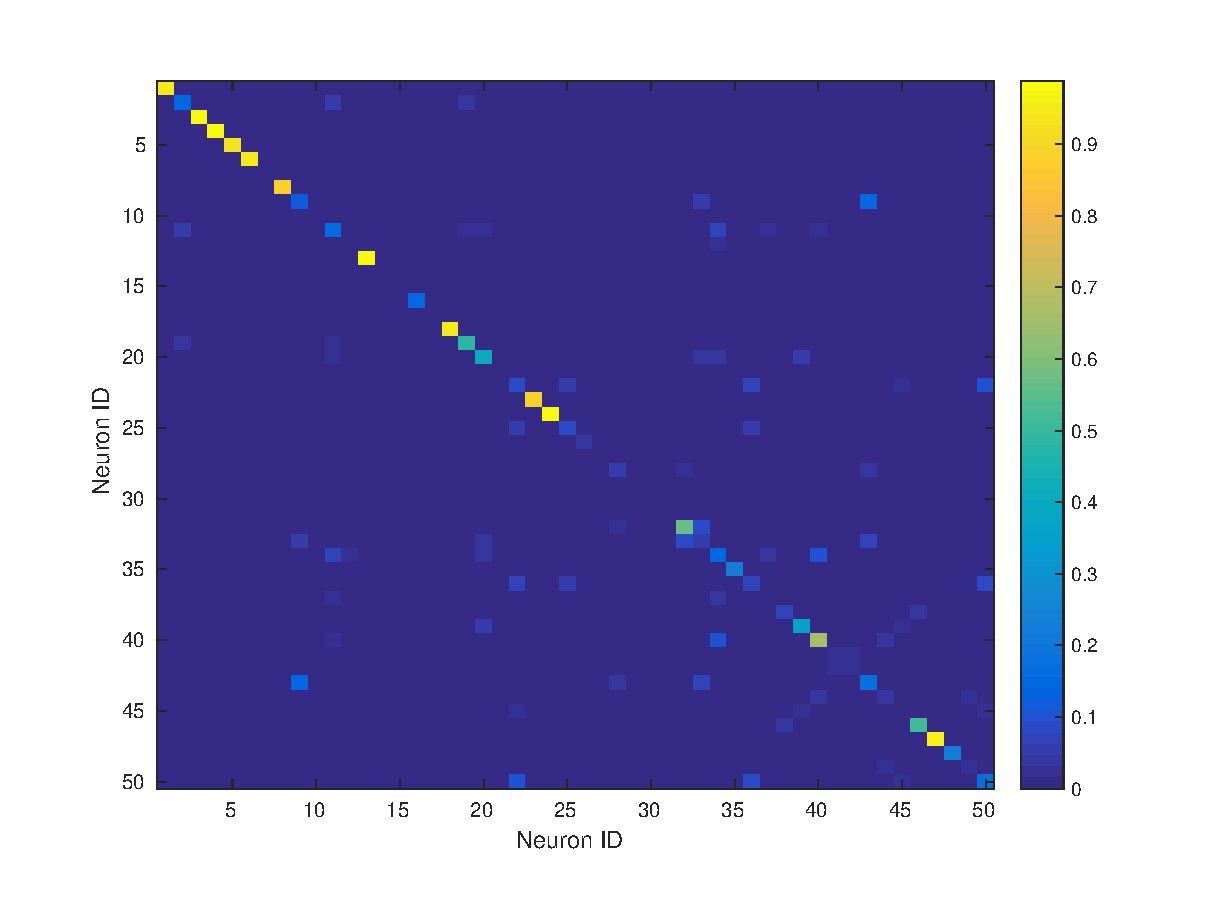
\includegraphics[width = \textwidth]{WW_6000Hz.eps}
\label{Compare: WW_STDP}
\caption{Multiplied weight matrix with STDP learning}
\end{subfigure}
\\
\begin{subfigure}[b]{0.49\textwidth}
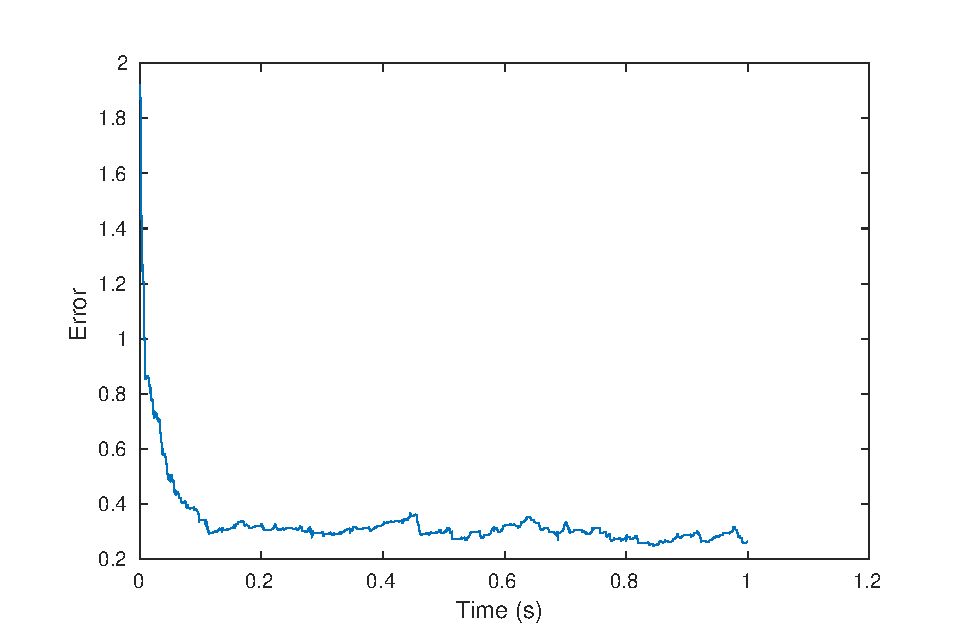
\includegraphics[width = \textwidth]{ErrorOverTime_6000Hz_Hebbian.eps}
\label{Compare: EoT_Hebbian}
\caption{Error over time of Hebbian plot}
\end{subfigure}
\,
\begin{subfigure}[b]{0.49\textwidth}
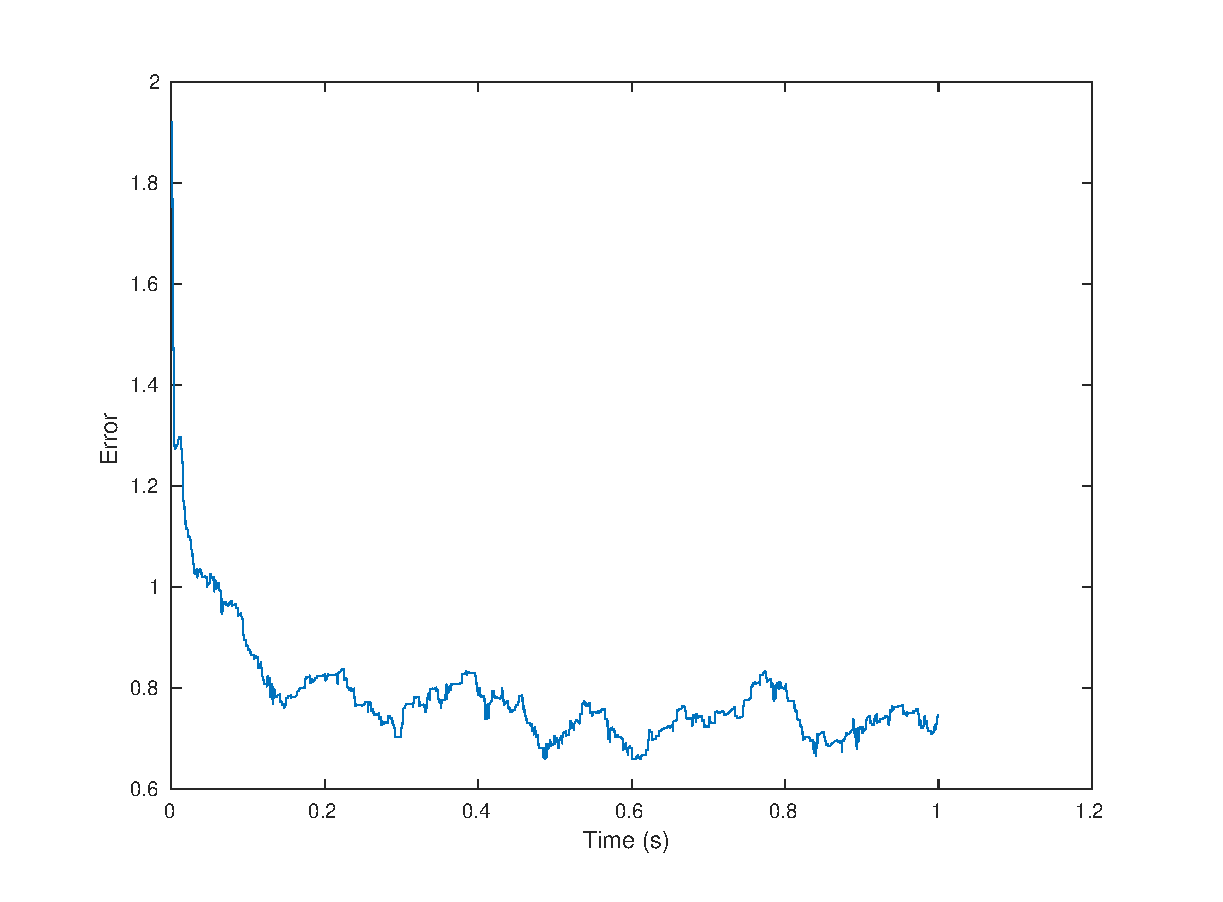
\includegraphics[width = \textwidth]{ErrorOverTime_6000Hz_normal.eps}
\label{Compare: EoT_STDP}
\caption{Error over time of STDP plot}
\end{subfigure}
\\
\begin{subfigure}[b]{0.49\textwidth}
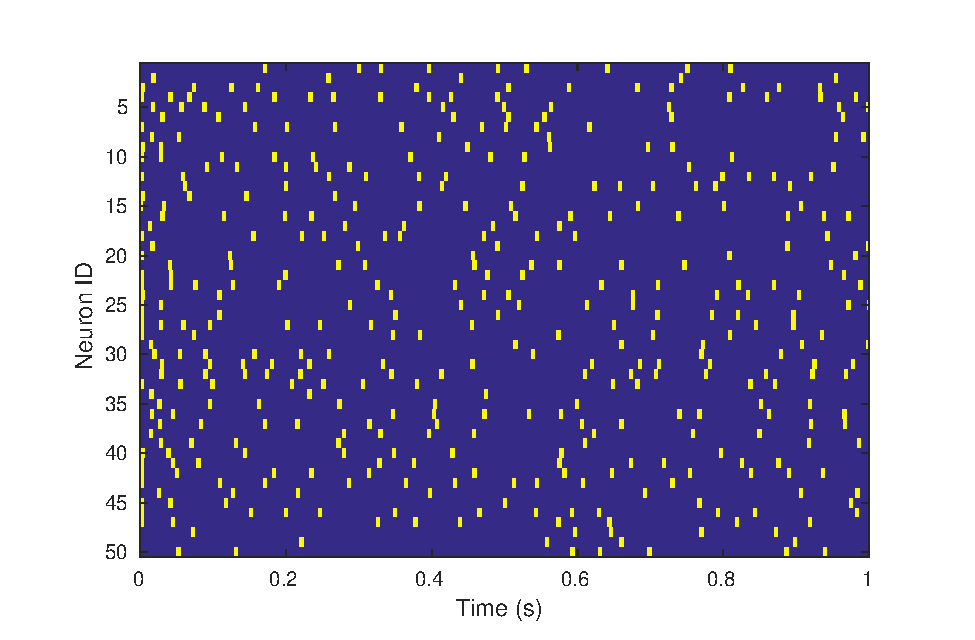
\includegraphics[width = \textwidth]{Burst_plot_6000Hz_Hebbian.eps}
\label{Compare: BH_Hebbian}
\caption{Burst history of Hebbian plot}
\end{subfigure}
\,
\begin{subfigure}[b]{0.49\textwidth}
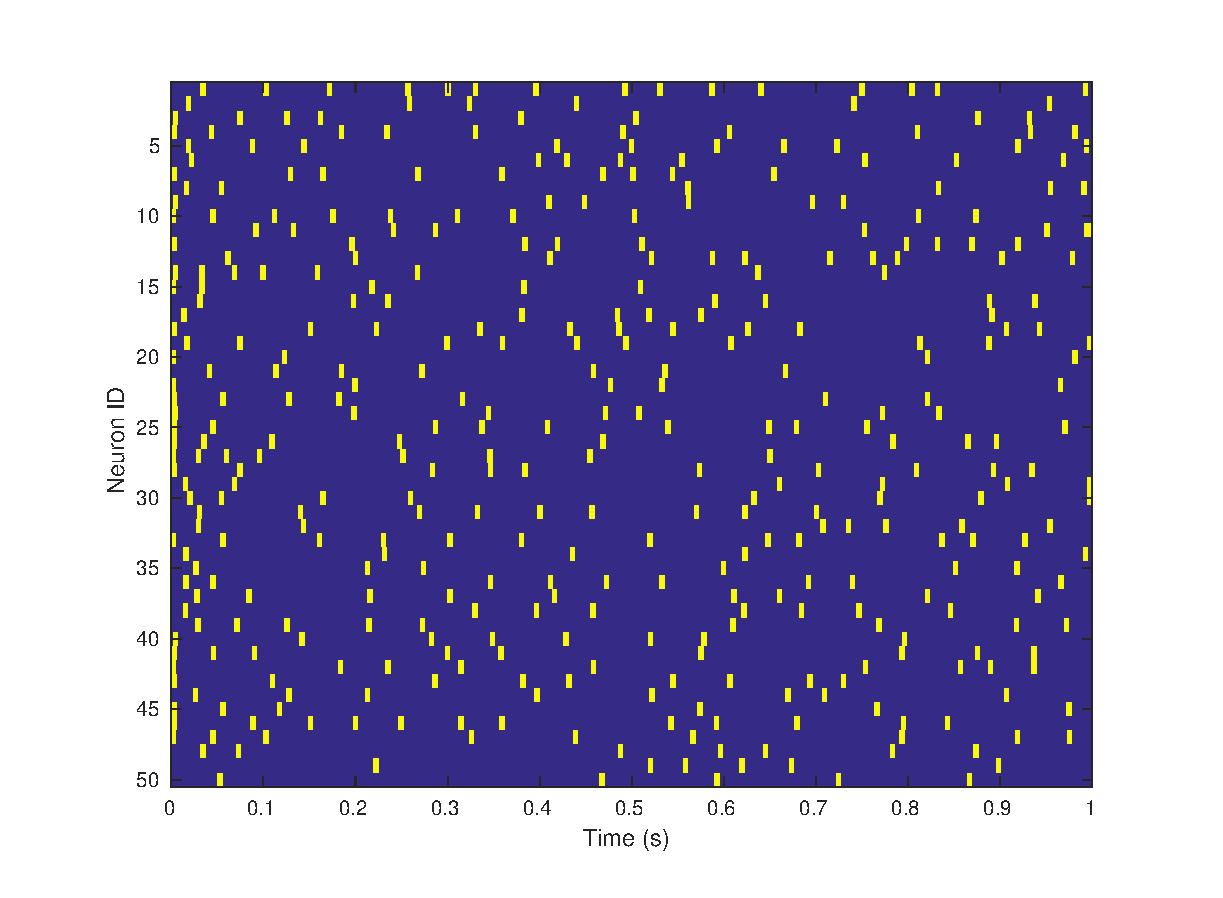
\includegraphics[width = \textwidth]{Burst_plot_6000Hz.eps}
\label{Compare: BH_STDP}
\caption{Burst history of STDP plot}
\end{subfigure}
\label{Compare}
\caption{Compare STDP to Hebbian}
\end{figure}
\end{itemize}

\section{Discussion}

Further improvements that could be made to our model and where this research could be taken.

\begin{figure}[H]
\centering
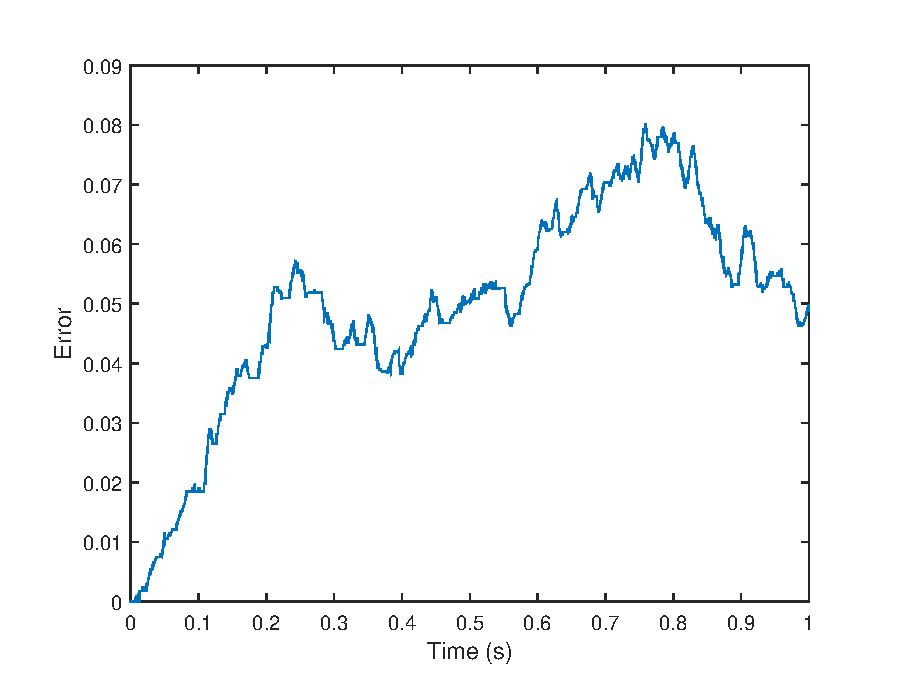
\includegraphics[width = \textwidth]{ErrorOverTime_6000Hz_perm_fixed.eps}
\label{EoT: fixed}
\caption{Here is a plot of error over time which was computed using the corrected algorithm presented in the methods section.}
\end{figure}

\section{Summary}

We generated a model similar to that used in \cite{Fiete} in an attempt to replicate the results from the paper. Our model did not work with the parameters provided by the paper, but we were able to generate a working IB model. In addition, while we did not see the synchronous regular firing observed in \cite{Fiete}, we were able to show partial convergence of weight matrices to scaled permutation matrices and limited synfiring chain behavior. We were also able to replicate these partial results with Hebbian learning instead of STDP learning. While our model had a number of minor flaws, it provided a nice start to verifying and testing the assertions of \cite{Fiete}.

\newpage

\bibliographystyle{plain}
\bibliography{Songbird_paper}


\end{document}